\documentclass[11pt,a4paper]{article}
\usepackage[T1]{fontenc}
\usepackage[utf8]{inputenc}
\usepackage[finnish]{babel}
\usepackage{lmodern}
\usepackage[a4paper,margin=2.8cm,top=2.6cm,bottom=3cm]{geometry}
\usepackage{amsmath,amssymb,amsthm,mathtools}
\usepackage{booktabs,array}
\usepackage[shortlabels]{enumitem}
\usepackage{microtype}
\usepackage{setspace}
\usepackage[parfill]{parskip}
\usepackage{xcolor}
\usepackage{tikz}
\usetikzlibrary{arrows.meta,positioning,calc}
\usepackage[most]{tcolorbox}
\usepackage[font=small,labelfont=bf,skip=6pt]{caption}
\usepackage[hidelinks]{hyperref}

\setstretch{1.12}
\widowpenalty=10000
\clubpenalty=10000
\setlist{itemsep=3pt,topsep=4pt}
\setlength{\parskip}{0.65\baselineskip}

\definecolor{sininen}{HTML}{0054E9}
\newtcolorbox{intuitio}{enhanced,breakable,colback=sininen!3,colframe=sininen!45,boxrule=0.4pt,
  leftrule=2.5pt,arc=1pt,left=9pt,right=9pt,top=5pt,bottom=5pt,
  title={Intuitio},fonttitle=\small\bfseries,coltitle=sininen!80!black,
  attach title to upper={\quad},before skip=8pt,after skip=10pt}

\theoremstyle{plain}
\newtheorem{lause}{Lause}
\newtheorem{lemma}{Lemma}
\newtheorem{propositio}{Propositio}
\newtheorem{seuraus}{Seuraus}
\theoremstyle{definition}
\newtheorem{maaritelma}{Määritelmä}
\newtheorem{oletus}{Oletus}
\theoremstyle{remark}
\newtheorem{huomautus}{Huomautus}

\newcommand{\E}{\mathbb{E}}
\renewcommand{\P}{\mathbb{P}}
\newcommand{\cC}{\mathcal{C}}
\newcommand{\cZ}{\mathcal{Z}}
\newcommand{\cT}{\mathcal{T}}
\newcommand{\cF}{\mathcal{F}}
\newcommand{\cB}{\mathcal{B}}
\newcommand{\cG}{\mathcal{G}}
\newcommand{\cH}{\mathcal{H}}
\newcommand{\cA}{\mathcal{A}}
\newcommand{\1}{\mathbf{1}}
\newcommand{\pol}[1]{\texttt{#1}}
\newcommand{\Bin}{\operatorname{Bin}}
\newcommand{\Poi}{\operatorname{Poisson}}
\newcommand{\Beta}{\operatorname{Beta}}
\DeclareMathOperator*{\argmax}{arg\,max}
% Taulukon rivit tiedostosta; primitiivinen \input toimii tabular-ympäristön sisällä.
\newcommand{\rivit}[1]{\csname @@input\endcsname #1 }

\title{\textbf{Tärinähavaintoihin perustuvan hiekoituksen\\ kohdistamisen hyöty}\\[6pt]
\large Liukkaussimulaattorin matemaattinen malli ja todistus}
\author{Elias Wuolijoki\\[2pt] \small Junction Turku 2026, If-haaste}
\date{18.10.2026}

\begin{document}
\maketitle

\begin{abstract}
\noindent
Tutkimme simulaattoria, jossa kävelijöiden puhelimet tunnistavat liukastumisia
tärinästä ja hiekoitus ohjataan näiden havaintojen perusteella. Turun keskustan
kulkuruuduilla on päivittäin vaihtuva piilevä liukkaus, jota kukaan ei näe
suoraan. Huolto ehtii hiekoittaa kerrallaan vain muutaman alueen, eikä samaa
aluetta saa hiekoittaa uudelleen, ennen kuin edellisen hiekoituksen vaikutus
on päättynyt.

Todistamme, että havainnoista laskettuun beta-binomiaaliseen posterioriin
perustuva kohdistus tuottaa odotusarvoltaan enintään yhtä paljon kaatumisia kuin
mikään havaintoja käyttämätön politiikka. Parhaaseen niistä verrattuna ero on
aidosti positiivinen täsmälleen silloin, kun liukkaus vaihtelee ruuduittain ja
tunnistus erottaa liukastumisen virhehälytyksestä. Tulokset koskevat simuloitua
maailmaa, eivät Turun todellisia katuja tai Ifin vahinkoja.
\end{abstract}

\vspace{4pt}
\setcounter{tocdepth}{1}
{\small\tableofcontents}
\newpage

% ---------------------------------------------------------------------------
\section{Johdanto}

\subsection{Kysymys}

Palveluidea on yksinkertainen. Kun kävelijä liukastuu, puhelimen
kiihtyvyysanturi huomaa sen. Jos tällaisia havaintoja kertyy samasta paikasta,
paikka on luultavasti liukas, ja hiekoitus kannattaa ohjata sinne.

Ajatus kuulostaa itsestään selvältä, mutta se ei ole sitä. Havainnot ovat
harvinaisia ja kohinaisia, ja osa niistä on virhehälytyksiä. Vilkkaalla
kadulla havaintoja kertyy jo pelkän kävelijämäärän vuoksi. Lisäksi huolto voi
yhtä hyvin kiertää alueita järjestyksessä tai hiekoittaa aina vilkkaimmat
kadut. Kysymys kuuluu siis:

\begin{center}
\emph{Onko tärinähavainnoista aitoa hyötyä verrattuna parhaaseen tapaan\\ hiekoittaa ilman niitä?}
\end{center}

\subsection{Vastaus lyhyesti}

Merkitään $J(\pi)$:llä politiikan $\pi$ odotettua kaatumisten määrää
tammikuussa 2026. Luvun~\ref{sec:lauseet} oletusten vallitessa todistamme ketjun
\begin{equation*}
  J(\pol{oraakkeli}) \;\le\; J(\pol{tuote}) \;<\; J(\pol{kulku})
  \;\le\; J(\pol{aikataulu}) \;\le\; J(\pol{ei\_huoltoa}).
\end{equation*}

Ketjun politiikat ovat seuraavat. \pol{tuote} käyttää tärinähavaintoja, ja
\pol{kulku} hiekoittaa vilkkaimmat alueet. \pol{aikataulu} kiertää alueita
järjestyksessä, ja \pol{oraakkeli} tuntee piilevän liukkauden. Ketjun tärkein
osa on keskimmäinen aito epäyhtälö: lauseen~\ref{la:sokea} mukaan \pol{kulku} on
paras mahdollinen politiikka, joka ei käytä havaintoja. Tärinähavainnot
voittavat siis \emph{jokaisen} havaintoja käyttämättömän säännön, eivät vain
satunnaisesti valittua vertailukohtaa.

Lauseen~\ref{la:valttamaton} mukaan ehdot ovat myös välttämättömiä: jos
liukkaus ei vaihtele ruuduittain tai jos tunnistus ei erota liukastumista
virhehälytyksestä, hyöty on täsmälleen nolla.

\subsection{Mitä tämä paperi ei väitä}

Lauseet koskevat simuloitua maailmaa, jossa palvelu tuntee mallin rakenteen ja
parametrit. Ne eivät osoita, että Turun kävelyväylät noudattaisivat tätä mallia,
että hiekoitus vähentäisi liukastumisia 80 prosenttia tai että puhelin
tunnistaisi liukastumisen kuvatulla tarkkuudella. Lauseet kertovat
järjestyksen, mutta erojen \emph{suuruus} riippuu oletuksista. Suuruutta
arvioidaan simuloimalla luvussa~\ref{sec:numeeriset}.

\subsection{Lukuohje}

Luku~\ref{sec:malli} kuvaa simuloidun maailman. Luku~\ref{sec:posteriori}
kertoo, miten palvelu päättelee liukkauden havainnoista. Luku~\ref{sec:hajotelma}
muuttaa kysymyksen hiekoituksen hyödystä kierroskohtaisiksi valintaongelmiksi,
ja luku~\ref{sec:lauseet} todistaa päätulokset. Luvut~\ref{sec:koodi}
ja~\ref{sec:numeeriset} liittävät tulokset koodiin ja numeroihin.

Kiireinen lukija voi lukea johdannon, kuvan~\ref{fig:malli}, lauseet
luvussa~\ref{sec:lauseet} intuitiolaatikoineen sekä taulukon~\ref{tab:oletus}.

% ---------------------------------------------------------------------------
\section{Simuloitu maailma}\label{sec:malli}

\subsection{Yleiskuva}

Kuva~\ref{fig:malli} näyttää, mitä yhdessä ruudussa tapahtuu yhden tunnin
aikana. Harmaat laatikot ovat simulaattorin piilossa pitämää totuutta, siniset
sitä, minkä palvelu näkee. Palvelu ei koskaan näe ruudun liukkautta eikä
kaatumisia, vain ohikulut ja tärinähavainnot.

\begin{figure}[ht]
\centering
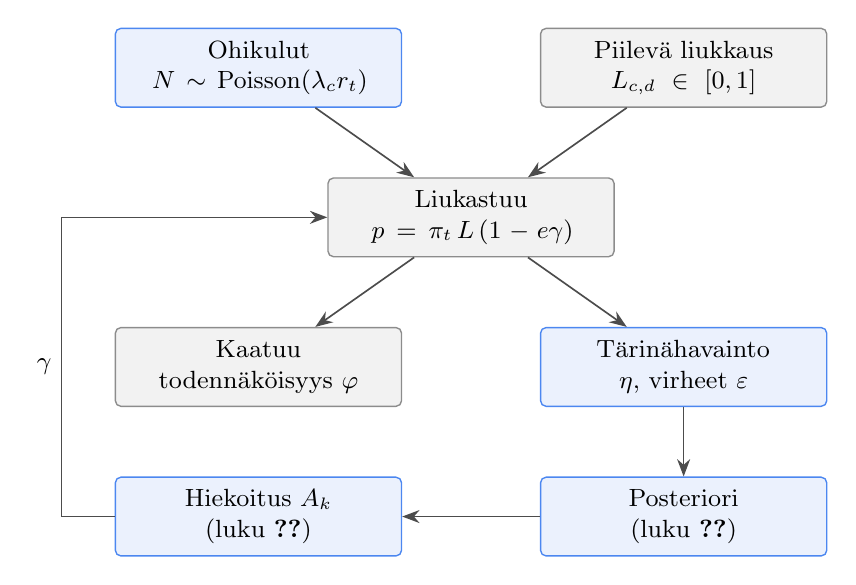
\begin{tikzpicture}[
  box/.style={draw,rounded corners=2pt,align=center,minimum height=10mm,text width=34mm,font=\small,line width=0.5pt},
  piilo/.style={box,fill=black!5,draw=black!45},
  nakyy/.style={box,fill=sininen!8,draw=sininen!70},
  nuoli/.style={-{Stealth[length=2.2mm]},line width=0.6pt,draw=black!70}]
  \node[nakyy] (N) at (0,0) {Ohikulut\\ $N \sim \Poi(\lambda_c r_t)$};
  \node[piilo] (L) at (5.4,0) {Piilevä liukkaus\\ $L_{c,d} \in [0,1]$};
  \node[piilo] (S) at (2.7,-1.9) {Liukastuu\\ $p = \pi_t\, L\, (1 - e\gamma)$};
  \node[piilo] (F) at (0,-3.8) {Kaatuu\\ todennäköisyys $\varphi$};
  \node[nakyy] (D) at (5.4,-3.8) {Tärinähavainto\\ $\eta$, virheet $\varepsilon$};
  \node[nakyy] (P) at (5.4,-5.7) {Posteriori\\ (luku~\ref{sec:posteriori})};
  \node[nakyy] (A) at (0,-5.7) {Hiekoitus $A_k$\\ (luku~\ref{sec:lauseet})};
  \draw[nuoli] (N) -- (S);
  \draw[nuoli] (L) -- (S);
  \draw[nuoli] (S) -- (F);
  \draw[nuoli] (S) -- (D);
  \draw[nuoli] (D) -- (P);
  \draw[nuoli] (P) -- (A);
  \draw[nuoli] (A.west) -- (-2.5,-5.7) -- node[midway,left,font=\small]{$\gamma$} (-2.5,-1.9) -- (S.west);
\end{tikzpicture}
\caption{Simulaattorin rakenne yhdessä ruudussa ja tunnissa. Harmaa: piilossa
oleva totuus. Sininen: palvelun näkemä tieto ja sen tekemät päätökset.
Hiekoitus $\gamma$ pienentää seuraavien tuntien liukastumisriskiä.}
\label{fig:malli}
\end{figure}

\subsection{Aika ja paikka}

Aika etenee tunneittain, $t \in \cT = \{1, \dots, T\}$, missä $T = 744$ on
tammikuun 2026 tuntien määrä. Tunti $t = 1$ on 1.1.2026 klo 00--01 Suomen aikaa.
Funktio $d(t)$ kertoo tunnin paikallisen vuorokauden; vuorokausi vaihtuu
keskiyöllä.

Tarkastelualue on $300 \times 300$ metrin neliö VPK-talon ympärillä
Turussa. Se jaetaan $10 \times 10$ metrin ruutuihin. Malliin kuuluvat ne
\[
  |\cC| = 85
\]
ruutua, jotka ovat enintään 5 metrin päässä jostakin neljästä käsin piirretystä
kävelyreitistä. Huolto toimii suuremmissa yksiköissä: $50 \times 50$ metrin
\emph{alueissa}, joita on $|\cZ| = 20$. Kuvaus $\zeta\colon \cC \to \cZ$ kertoo,
mihin alueeseen ruutu kuuluu, ja $\cC_z = \zeta^{-1}(z)$ on alueen $z$ ruutujen
joukko.

\subsection{Kulkeminen ja sää}

Seuraavat suureet ovat deterministisiä, ja kaikki politiikat tuntevat ne.

\textbf{Kulkemisen perustaso.} Ruudun $c$ tunnittainen ohikulkujen perustaso
$\lambda_c > 0$ on sen lähellä kulkevien reittien oletettujen tuntimäärien
summa. Alueen perustaso on $\lambda(z) = \sum_{c \in \cC_z} \lambda_c$.

\textbf{Vuorokausirytmi.} Olkoon $h_t$ tunnin $t$ alkamiskellonaika. Kulkeminen
painottuu aamuun ja iltapäivään:
\[
  r_t = \Bigl(0{,}1 + 0{,}8\, e^{-((h_t - 8)/2)^2} + 0{,}9\, e^{-((h_t - 17)/3)^2}\Bigr)
  \cdot
  \begin{cases} 0{,}7, & \text{viikonloppuna},\\ 1, & \text{arkena}. \end{cases}
\]

\textbf{Sää.} Turku Artukaisen mitatuista tuntikeskiarvoista (lämpötila $T_t$,
lumensyvyys $s_t$, sade $q_t$) lasketaan sääkerroin
\[
  w_t = 0{,}7 + 1{,}2 \cdot \1\{-3 \le T_t \le 1\} + 0{,}6 \cdot \1\{s_t > 0\}
        + 0{,}5 \cdot \1\{q_t > 0,\ T_t < 1\},
\]
joka on välillä $[0{,}7;\ 3{,}0]$. Liukastumisen perustodennäköisyys
ohikulkua kohti on $\pi_t = p_0 w_t$, missä $p_0 = 0{,}01$.

Sääkerroin on simulaattorin oma kokeellinen sääntö, eikä sitä ole kalibroitu
tienpinnan havaintoihin. Se kuvaa yksinkertaisesti sitä, että nollan tienoilla
on liukkaampaa kuin kovalla pakkasella.

\subsection{Piilevä liukkaus}

Jokaisella ruudulla on jokaisena päivänä oma \emph{piilevä liukkaus}
$L_{c,d} \in [0,1]$. Se kuvaa asioita, joita sää ei kerro: varjoa, kaltevuutta,
räystäältä tippuvaa vettä tai kiillottunutta jäätä. Arvo $L = 1$ on liukkain
mahdollinen ruutu ja $L \approx 0$ käytännössä pitävä.

Liukkauden jakauma halutaan voimakkaasti vinoksi: suurin osa ruuduista on
pitäviä, mutta muutama on todella liukas. Beta-jakauma $\Beta(a,b)$ pienellä
parametrilla $a$ on tällainen. Laskennan tarkkuuden vuoksi jakauma
diskretoidaan.

\begin{maaritelma}[Liukkaustasot]\label{maar:tasot}
Olkoot $a, b > 0$ ja $G \in \mathbb{N}$. Olkoon $B \sim \Beta(a,b)$ ja $F$ sen
kertymäfunktio. Jaetaan väli $[0,1]$ $G$:hen yhtä todennäköiseen osaan
pisteillä $q_j = F^{-1}(j/G)$, $j = 0, \dots, G$, ja asetetaan
\[
  \ell_g = \E\bigl[B \mid q_{g-1} < B \le q_g\bigr], \qquad g = 1, \dots, G.
\]
Liukkauden jakauma on tasainen jakauma tasoilla:
$\nu = \frac{1}{G} \sum_{g=1}^{G} \delta_{\ell_g}$. Sen odotusarvo on
$\mu = \sum_g \nu_g \ell_g$.
\end{maaritelma}

\begin{lemma}\label{le:tasot}
Määritelmän~\ref{maar:tasot} tasoille pätee:
\begin{enumerate}[(i)]
  \item $\ell_g = G \cdot \frac{a}{a+b} \bigl(I_{q_g}(a+1, b) - I_{q_{g-1}}(a+1, b)\bigr)$,
  missä $I_x$ on säännöllistetty epätäydellinen beetafunktio;
  \item $0 < \ell_1 < \ell_2 < \dots < \ell_G < 1$;
  \item $\mu = a/(a+b)$, eli diskretointi säilyttää keskiarvon.
\end{enumerate}
\end{lemma}

\begin{proof}
Beetatiheydelle pätee $x f_{a,b}(x) = \frac{a}{a+b} f_{a+1,b}(x)$, koska
$B(a+1,b)/B(a,b) = a/(a+b)$. Jokaisen välin todennäköisyys on $1/G$, joten
\[
  \ell_g = G \int_{q_{g-1}}^{q_g} x f_{a,b}(x)\,dx
         = G \frac{a}{a+b} \int_{q_{g-1}}^{q_g} f_{a+1,b}(x)\,dx,
\]
mikä on kohta (i).

Tiheys on positiivinen välillä $(0,1)$. Siksi $0 = q_0 < q_1 < \dots < q_G = 1$,
ja välin ehdollinen odotusarvo on aidosti välin sisällä:
$q_{g-1} < \ell_g < q_g$. Tästä seuraa kohta (ii).

Kohta (iii) on kokonaisodotusarvon kaava:
$\mu = \sum_g \frac{1}{G}\, \E[B \mid \text{väli } g] = \E B = a/(a+b)$.
\end{proof}

\textbf{Oletusarvot.} Simulaattorissa $a = 1/4$, $b = 1$ ja $G = 40$. Kun
$b = 1$, kertymäfunktio on yksinkertaisesti $F(x) = x^{a}$, ja tasoille saadaan
suljettu muoto
\[
  \ell_g = \frac{g^5 - (g-1)^5}{5\, G^4}.
\]
Keskiarvo on $\mu = 0{,}2$, liukkain taso $\ell_{40} \approx 0{,}951$ ja
pitävin $\ell_1 \approx 7{,}8 \cdot 10^{-8}$. Jatkuvassa jakaumassa
$\P(B < 0{,}004) \approx 0{,}25$ ja $\P(B > 0{,}5) \approx 0{,}16$.

\begin{intuitio}
Neljännes ruuduista on käytännössä pitäviä, ja joka kuudes on hyvin liukas.
Tällainen maailma palkitsee kohdistamisen: jos tietäisi, missä liukkaat ruudut
ovat, hiekoitus osuisi niihin moninkertaisella teholla.
\end{intuitio}

Liukkaus muuttuu päivittäin. Pysyvyysparametri $\rho$ kertoo, kuinka
todennäköisesti eilinen tilanne säilyy.

\begin{maaritelma}[Liukkauden dynamiikka]\label{maar:dynamiikka}
Olkoon $\rho \in [0, 1]$. Jokaiselle ruudulle $c$ arvotaan $L_{c,1} \sim \nu$.
Seuraavana päivänä $L_{c,d+1} = L_{c,d}$ todennäköisyydellä $\rho$; muuten
$L_{c,d+1}$ arvotaan uudelleen jakaumasta $\nu$. Kaikki arvonnat ovat
riippumattomia ruutujen ja päivien välillä.
\end{maaritelma}

\begin{lemma}\label{le:markov}
Kaikilla $c$, $d$ ja $j \ge 0$ pätee $L_{c,d} \sim \nu$ sekä
\[
  \E[L_{c,d+j} \mid L_{c,1}, \dots, L_{c,d}] = \mu + \rho^j (L_{c,d} - \mu).
\]
\end{lemma}

\begin{proof}
Siirtymäydin on $P(\ell_g, \ell_h) = \rho\, \1\{g = h\} + (1-\rho)\nu_h$.
Koska $\nu P = \rho \nu + (1-\rho)\nu = \nu$ ja alkujakauma on $\nu$, induktio
antaa $L_{c,d} \sim \nu$ kaikilla $d$. Markovin ominaisuuden nojalla
$\E[L_{c,d+1} \mid L_{c,\le d}] = \rho L_{c,d} + (1-\rho)\mu$, ja väite seuraa
induktiolla luvun $j$ suhteen.
\end{proof}

Simulaattorin oletus on $\rho = 0$: jokaisen ruudun liukkaus arvotaan joka
päivä uudelleen. Silloin edellisen päivän havainnoista ei ole hyötyä, ja
palvelun on opittava päivän tilanne saman päivän havainnoista.

\subsection{Ohikulut, liukastumiset ja havainnot}

Kaikki satunnaisuus rakennetaan yhdelle todennäköisyysavaruudelle, jotta
riippumattomuusväitteet ovat täsmällisiä.

\begin{maaritelma}[Todennäköisyysavaruus]\label{maar:avaruus}
Todennäköisyysavaruudella $(\Omega, \cA, \P)$ on seuraavat keskenään
riippumattomat satunnaissuureiden perheet:
\begin{enumerate}[(a)]
  \item ohikulut $N_{c,t} \sim \Poi(\lambda_c r_t)$, riippumattomia kaikilla $(c,t)$;
  \item liukkauden arvonnat määritelmän~\ref{maar:dynamiikka} mukaisesti;
  \item ohikulkukohtaiset tasajakautuneet suureet $U_{c,t,i,j}$, missä
  $i \in \mathbb{N}$ ja $j \in \{1, 2, 3\}$;
  \item sokean politiikan mahdollinen satunnaistus $V$ (määritelmä~\ref{maar:politiikka}).
\end{enumerate}
Merkitään tunnin $t$ satunnaisuutta $\Psi_t = (N_{c,t}, U_{c,t,i,j})_{c, i, j}$
ja koko liukkausprosessia $L$. Tällöin $L, V, \Psi_1, \Psi_2, \dots$ ovat
riippumattomia.
\end{maaritelma}

Olkoon $\gamma_{c,t} \in \{0,1\}$ tieto siitä, onko ruudun $c$ alue
hiekoitettu tunnilla $t$; se määräytyy politiikasta
(luku~\ref{sec:huolto}). Mallin muut parametrit ovat
\begin{center}
\begin{tabular}{@{}ll@{}}
$e \in [0,1]$ & hiekoituksen teho, \\
$\varphi$ & kaatumisen todennäköisyys liukastumisesta, \\
$\eta$ & tunnistuksen herkkyys, \\
$\varepsilon$ & virhehavainnon todennäköisyys ohikulkua kohti.
\end{tabular}
\end{center}

Liukastumisen todennäköisyys ohikulkua kohti on
\begin{equation}\label{eq:p}
  p_{c,t} = \pi_t\, L_{c,d(t)}\, (1 - e\,\gamma_{c,t}).
\end{equation}
Oletamme, että $\pi_t \ell_G < 1$ kaikilla $t$; oletusarvoilla
$\max_t \pi_t \ell_G \le 0{,}03 \cdot 0{,}951$.

Jokainen ohikulku $i = 1, \dots, N_{c,t}$ käsitellään erikseen:
\begin{itemize}
  \item ohikulku johtaa liukastumiseen, jos $U_{c,t,i,1} \le p_{c,t}$;
  \item liukastuminen johtaa kaatumiseen, jos $U_{c,t,i,2} \le \varphi$;
  \item tärinätunnistus hälyttää, jos liukastuminen tapahtui ja
  $U_{c,t,i,3} \le \eta$, tai jos sitä ei tapahtunut ja $U_{c,t,i,3} \le \varepsilon$.
\end{itemize}
Liukastumisten, kaatumisten ja havaintojen määriä merkitään $S_{c,t}$,
$F_{c,t}$ ja $D_{c,t}$.

\begin{lemma}[Havaintojen ja kaatumisten jakauma]\label{le:havainnot}
Olkoon $\cG_t = \sigma(L, V, \Psi_1, \dots, \Psi_{t-1}, N_{\cdot,t})$, ja olkoon
$\gamma_{\cdot,t}$ $\sigma(L, V, \Psi_{<t})$-mitallinen. Tällöin ehdolla $\cG_t$
suureet $D_{c,t}$, $c \in \cC$, ovat riippumattomia, ja
\[
  D_{c,t} \sim \Bin\bigl(N_{c,t},\, \theta_t(L_{c,d(t)}, \gamma_{c,t})\bigr),
  \qquad
  \theta_t(\ell, \gamma) = \varepsilon + (\eta - \varepsilon)\, \pi_t\, \ell\, (1 - e \gamma).
\]
Lisäksi $\E[F_{c,t} \mid \cG_t] = \varphi\, N_{c,t}\, p_{c,t}$.
\end{lemma}

\begin{proof}
Ehdolla $\cG_t$ todennäköisyys $p_{c,t}$ on tunnettu, ja suureet
$U_{c,t,\cdot,\cdot}$ ovat riippumattomia $\cG_t$:stä. Yksittäinen ohikulku
tuottaa hälytyksen todennäköisyydellä
$p_{c,t}\eta + (1 - p_{c,t})\varepsilon = \theta_t(L_{c,d(t)}, \gamma_{c,t})$, ja
ohikulut ovat keskenään riippumattomia. Samoin ohikulku johtaa kaatumiseen
todennäköisyydellä $p_{c,t}\varphi$.
\end{proof}

\begin{intuitio}
Hälytyksen todennäköisyys $\theta$ on liukkauden \emph{affiini} funktio. Kun
$\eta > \varepsilon$, liukkaampi ruutu tuottaa keskimäärin enemmän hälytyksiä
ohikulkua kohti. Tämä on ainoa kanava, jota pitkin palvelu saa tietoa
liukkaudesta.
\end{intuitio}

\begin{huomautus}[Toteutus ja yhteiset satunnaisluvut]\label{hu:crn}
Koodi ei arvo jokaista ohikulkua erikseen. Se arpoo summat $S$, $F$ ja $D$
suoraan binomijakaumista käänteisen kertymäfunktion avulla, ja jokainen
politiikka saa saman tasajakautuneen luvun. Ehdolla $(N_{c,t}, p_{c,t})$
summien jakauma on sama kuin yllä, joten jokaisen politiikan oma jakauma on
täsmälleen tämä malli. Yhteiset satunnaisluvut kytkevät politiikat toisiinsa
vain, jotta niiden erotus voidaan estimoida pienemmällä varianssilla.
\end{huomautus}

\subsection{Huolto ja päällekkäisen hiekoituksen kielto}\label{sec:huolto}

\begin{maaritelma}[Huoltokierrokset]\label{maar:huolto}
Olkoot $\Delta$, $H$ ja $K$ positiivisia kokonaislukuja: huoltoväli,
vaikutusaika ja kerralla hiekoitettavien alueiden määrä. Kierrokset alkavat
tunneilla $\tau_k = 1 + (k-1)\Delta$, $k = 1, \dots, \kappa$, missä
$\kappa = \lceil T/\Delta \rceil$. Kierroksen $k$ \emph{vaikutusikkuna} on
\[
  W_k = \{\tau_k, \dots, \tau_k + H - 1\} \cap \cT.
\]
Kierroksella valitaan joukko $A_k \subseteq \cZ$, jossa $|A_k| = K$. Valinnan
saa tehdä vain kelpoisista alueista:
\[
  A_k \subseteq E_k := \cZ \setminus \bigcup\bigl\{A_j : j < k,\ \tau_j + H > \tau_k\bigr\}.
\]
Tämä on \emph{päällekkäisen hiekoituksen kielto}: aluetta ei valita, jos sen
edellinen hiekoitus on yhä voimassa. Hiekoitustieto on
$\gamma_{c,t} = \1\{\exists k : \zeta(c) \in A_k,\ t \in W_k\}$.
\end{maaritelma}

\begin{lemma}\label{le:erilliset}
Kiellon voimassa ollessa saman alueen vaikutusikkunat ovat erillisiä. Siksi
\[
  \gamma_{c,t} = \sum_{k} \1\{\zeta(c) \in A_k\}\, \1\{t \in W_k\}.
\]
\end{lemma}

\begin{proof}
Olkoot $j < k$ ja $z \in A_j \cap A_k$. Kelpoisuuden mukaan $\tau_j + H \le \tau_k$,
joten $\max W_j < \tau_k = \min W_k$. Summassa on siis enintään yksi nollasta
poikkeava termi.
\end{proof}

\subsection{Informaatio, politiikat ja tavoite}

Palvelu näkee ohikulut ja tärinähavainnot sitä mukaa kuin ne tapahtuvat. Sen
informaatio tunnin $t$ lopussa on
\[
  \cF_t = \sigma\bigl(N_{c,s},\, D_{c,s} : c \in \cC,\ s \le t\bigr),
\]
ja $\cF_0$ on triviaali.

\begin{maaritelma}[Politiikka]\label{maar:politiikka}
\emph{Politiikka} on sääntö, jonka valinta $A_k$ on $\cF_{\tau_k - 1}$-mitallinen
ja kelpoinen: päätös tehdään ennen kierroksen alkua kaikella siihen asti
kertyneellä tiedolla. Koska havainnot riippuvat aiemmista hiekoituksista,
informaatio riippuu politiikasta; merkitään sitä tarvittaessa $\cF^\pi_t$.
\begin{itemize}
  \item Politiikka on \emph{sokea}, jos $A_k$ on mitallinen $\sigma$-algebran
  $\cB_{\tau_k - 1} \vee \sigma(V)$ suhteen, missä
  $\cB_t = \sigma(N_{c,s} : s \le t)$. Sokea politiikka voi käyttää kellonaikaa,
  säätä, ohikulkuja ja omaa satunnaistustaan, mutta ei tärinähavaintoja.
  \item \emph{Oraakkelin} informaatio on
  $\cH_k = \sigma\bigl(L_{\cdot,d} : d \le d(\tau_k);\ \Psi_s : s < \tau_k\bigr)$.
  Se tuntee kuluvan päivän liukkauden mutta ei tulevaa satunnaisuutta.
  Jokaisella politiikalla $\cF^\pi_{\tau_k - 1} \subseteq \cH_k$.
\end{itemize}
\end{maaritelma}

\begin{maaritelma}[Tavoite]
Politiikan $\pi$ arvo on odotettu kaatumisten määrä
\[
  J(\pi) = \E^\pi\Bigl[\sum_{c \in \cC} \sum_{t \in \cT} F_{c,t}\Bigr].
\]
\end{maaritelma}

Simulaattorin sarake \texttt{expected\_falls} on $\sum_{c,t} \varphi N_{c,t} p_{c,t}$.
Lemman~\ref{le:havainnot} ja torniominaisuuden nojalla sen odotusarvo on
$J(\pi)$. Se on siis harhaton estimaattori, jonka varianssi on pienempi kuin
arvottujen kaatumisten.

\begin{table}[ht]
\centering
\small
\begin{tabular}{@{}l l@{}}
\toprule
Merkintä & Merkitys \\
\midrule
$c \in \cC$, $z \in \cZ$ & ruutu ($10 \times 10$ m) ja huoltoalue ($50 \times 50$ m) \\
$t$, $d(t)$ & tunti ja sen vuorokausi \\
$\lambda_c$, $r_t$, $\pi_t$ & kulkemisen perustaso, vuorokausirytmi, säästä johtuva perusriski \\
$L_{c,d}$, $\ell_g$, $\nu$, $\mu$ & piilevä liukkaus, sen tasot, jakauma ja keskiarvo \\
$\rho$ & liukkauden pysyvyys päivästä toiseen \\
$N$, $S$, $F$, $D$ & ohikulut, liukastumiset, kaatumiset, tärinähavainnot \\
$e$, $\varphi$, $\eta$, $\varepsilon$ & hiekoituksen teho, kaatumisosuus, herkkyys, virhehälytykset \\
$\Delta$, $H$, $K$ & huoltoväli, vaikutusaika, alueita kierroksella \\
$A_k$, $W_k$, $\gamma_{c,t}$ & kierroksen valinta, vaikutusikkuna, hiekoitustieto \\
$\cF_t$, $\cB_t$, $\cH_k$ & palvelun, sokean politiikan ja oraakkelin informaatio \\
$J(\pi)$ & odotettu kaatumisten määrä \\
\bottomrule
\end{tabular}
\caption{Keskeiset merkinnät.}
\label{tab:merkinnat}
\end{table}

% ---------------------------------------------------------------------------
\section{Mitä palvelu tietää: beta-binomiaalinen posteriori}\label{sec:posteriori}

Palvelu ei näe liukkautta, mutta se voi päätellä sen havainnoista Bayesin
kaavalla. Tässä luvussa näytetään, että päättely jakautuu ruuduittain ja on
laskettavissa yksinkertaisella rekursiolla.

Oletetaan, että politiikka on \emph{deterministinen}: valinta $A_k$ on
havaintohistorian deterministinen funktio. Kaikki koodin politiikat ovat
tällaisia, ja tasapelit ratkaistaan alueen numeron mukaan.

\begin{propositio}[Suodin]\label{pr:suodin}
Ehdolla $\cF_t$ ruutujen liukkausketjut $(L_{c,d})_d$, $c \in \cC$, ovat
riippumattomia. Jokaisen ruudun suodatusjakauma
\[
  w_{c,g}(t) = \P\bigl(L_{c,d(t)} = \ell_g \mid \cF_t\bigr)
\]
saadaan rekursiolla:
\begin{enumerate}[(i)]
  \item Aluksi $w_c = \nu$. Kun päivä vaihtuu, jakauma ennustetaan seuraavalle
  päivälle: $w_c \mapsto \rho\, w_c + (1 - \rho)\nu$.
  \item Tunnin $t$ havainnot päivittävät jakaumaa:
  \[
    w_{c,g}(t) \;\propto\; w_{c,g}(t-1)\; \theta_t(\ell_g, \gamma_{c,t})^{D_{c,t}}
    \bigl(1 - \theta_t(\ell_g, \gamma_{c,t})\bigr)^{N_{c,t} - D_{c,t}}.
  \]
\end{enumerate}
Liukkauden posteriorin odotusarvo on $m_c(t) = \sum_g w_{c,g}(t)\, \ell_g$.
\end{propositio}

\begin{proof}
Olkoon $h = (n_{c,s}, \delta_{c,s})_{c \in \cC,\, s \le t}$ havaintohistoria ja
$l = (l_{c,d})$ liukkauspolku. Koska politiikka on deterministinen,
$\gamma_{c,s} = \gamma_{c,s}(h_{<s})$. Ehdollistamalla tunti kerrallaan
lemman~\ref{le:havainnot} avulla saadaan
\[
  \P(N_{\le t} = n,\ D_{\le t} = \delta \mid L = l)
  = \prod_{s \le t} \prod_{c} \Poi(n_{c,s}; \lambda_c r_s)
    \binom{n_{c,s}}{\delta_{c,s}}\, \theta_s^{\delta_{c,s}} (1 - \theta_s)^{n_{c,s} - \delta_{c,s}},
\]
missä $\theta_s = \theta_s\bigl(l_{c,d(s)}, \gamma_{c,s}(h_{<s})\bigr)$.

Polun $l$ funktiona tämä on tulo ruutukohtaisista tekijöistä. Myös priori on
tulomuotoinen, koska ruutujen ketjut ovat riippumattomia. Siksi posteriori on
tulomuotoinen, ja kunkin ruudun posteriori on piilo-Markov-mallin posteriori.
Mallin siirtymäydin on lemman~\ref{le:markov} $P$, ja tunnin havainnon
todennäköisyys on yllä oleva binomitekijä. Eteenpäin-algoritmi antaa kohdat (i)
ja (ii); kohdan (i) ennuste on $wP = \rho w + (1 - \rho)\nu$.
\end{proof}

Koodissa päivitys on funktio \texttt{paivita\_posteriori}. Simulaattori arpoo
liukkauden samasta diskreetistä jakaumasta $\nu$, jota palvelu käyttää
priorina. Laskettu posteriori on siksi tarkka, ei approksimaatio.

Nimitys \emph{beta-binomiaalinen} tulee seuraavasta erikoistapauksesta, jossa
priori on jatkuva beetajakauma ja hälytys kertoo liukkauden suoraan.

\begin{propositio}[Konjugaatti erikoistapaus]\label{pr:konjugaatti}
Olkoon priori jatkuva $\Beta(a,b)$, ja olkoon $\theta = \ell$ eli $\eta = 1$,
$\varepsilon = 0$ ja $\pi_s(1 - e\gamma) = 1$. Jos saman päivän aikana on
$n = \sum_s N_s$ ohikulkua ja $y = \sum_s D_s$ havaintoa, posteriori on
$\Beta(a + y,\ b + n - y)$, ja
\[
  \E[L \mid \text{data}] = \frac{a + y}{a + b + n}
  = \underbrace{\frac{a + b}{a + b + n}}_{\text{priorin paino}}\cdot\frac{a}{a+b}
  \;+\; \underbrace{\frac{n}{a + b + n}}_{\text{datan paino}}\cdot\frac{y}{n}.
\]
Lisäksi $y$:n reunajakauma ehdolla $n$ on beta-binomijakauma $\mathrm{BB}(n, a, b)$.
\end{propositio}

\begin{proof}
Posteriorin tiheys on verrannollinen lausekkeeseen
$\ell^{a-1}(1-\ell)^{b-1} \cdot \ell^{y}(1-\ell)^{n-y}$, joka on
$\Beta(a+y, b+n-y)$-tiheyden ydin. Reunajakauma on
$\binom{n}{y} B(a+y, b+n-y)/B(a,b)$, mikä on beta-binomijakauman määritelmä.
\end{proof}

\begin{intuitio}
Priori $\Beta(a,b)$ vastaa $a + b$ kuviteltua ohikulkua, joista $a$ on johtanut
havaintoon. Posteriorin odotusarvo on painotettu keskiarvo: vähällä datalla se
pysyy lähellä priorin keskiarvoa, paljolla datalla se lähestyy havaittua
osuutta $y/n$. Yksi hälytys yhdestä ohikulusta ei siis tee ruudusta liukasta.

Simulaattorissa $\theta$ on liukkauden affiini funktio, joten posteriori ei ole
beetamuotoinen. Siksi se lasketaan tarkasti tasojen $\ell_1, \dots, \ell_G$
hilassa. Tarkistus \texttt{tarkista\_tammikuu.R} varmistaa, että hilalaskenta
tuottaa proposition~\ref{pr:konjugaatti} tuloksen, kun $G = 4000$.
\end{intuitio}

% ---------------------------------------------------------------------------
\section{Hyödyn hajotelma}\label{sec:hajotelma}

Kuukauden kaatumismäärä on monimutkainen satunnaissuure: jokainen hiekoitus
vaikuttaa tuleviin liukastumisiin, havaintoihin ja päätöksiin. Tässä luvussa
näytetään, että odotusarvo kuitenkin jakautuu siististi kierroskohtaisiksi
termeiksi.

Määritellään alueen $z$ \emph{riskimassa} kierroksen $k$ vaikutusikkunassa sekä
sen deterministinen vastine, \emph{altistus}:
\[
  R_{z,k} = \sum_{c \in \cC_z} \sum_{t \in W_k} N_{c,t}\, \pi_t\, L_{c,d(t)},
  \qquad
  \Lambda_{z,k} = \lambda(z)\, \kappa_k, \quad \kappa_k = \sum_{t \in W_k} r_t \pi_t .
\]
Riskimassa on se määrä liukastumisriskiä, jonka hiekoitus voisi poistaa.
Se ei riipu politiikasta, koska se on ohikulkujen ja liukkauden funktio.

\begin{propositio}[Hyödyn hajotelma]\label{pr:hajotelma}
Olkoon $\cG_k$ mikä tahansa $\sigma$-algebra, jonka suhteen $A_k$ on mitallinen.
Jokaiselle kieltoa noudattavalle politiikalle pätee
\[
  J(\pi) = \mathsf{B} - e \varphi \sum_{k=1}^{\kappa}
  \E^\pi\Bigl[\sum_{z \in A_k} \E[R_{z,k} \mid \cG_k]\Bigr],
  \qquad
  \mathsf{B} = \varphi \mu \sum_{c,t} \lambda_c r_t \pi_t = J(\pol{ei\_huoltoa}).
\]
\end{propositio}

\begin{proof}
\emph{Vaihe 1.} Lemman~\ref{le:havainnot} ja torniominaisuuden nojalla
$\E F_{c,t} = \varphi\,\E\bigl[N_{c,t}\, \pi_t L_{c,d(t)} (1 - e\gamma_{c,t})\bigr]$.

\emph{Vaihe 2.} Lemman~\ref{le:erilliset} mukaan hiekoitettu osa voidaan
ryhmitellä kierroksittain:
\[
  \sum_{c,t} N_{c,t}\pi_t L_{c,d(t)} \gamma_{c,t}
  = \sum_k \sum_{z \in A_k} \sum_{c \in \cC_z} \sum_{t \in W_k} N_{c,t}\pi_t L_{c,d(t)}
  = \sum_k \sum_{z \in A_k} R_{z,k}.
\]

\emph{Vaihe 3.} Koska $N \perp L$ ja $L_{c,d} \sim \nu$, on
$\E[N_{c,t}\pi_t L_{c,d(t)}] = \lambda_c r_t \pi_t \mu$, mistä saadaan $\mathsf{B}$.

\emph{Vaihe 4.} Lopuksi
$\E[\1\{z \in A_k\} R_{z,k}] = \E\bigl[\1\{z \in A_k\}\,\E[R_{z,k} \mid \cG_k]\bigr]$,
koska $\1\{z \in A_k\}$ on $\cG_k$-mitallinen ja $R_{z,k} \ge 0$ on integroituva.
\end{proof}

\begin{intuitio}
Kielto takaa, ettei sama ruutu-tunti koskaan hyödy kahdesta hiekoituksesta.
Silloin hyöty on summa kierroksittaisista valinnoista: kuinka paljon
riskimassaa valitut alueet sisältävät \emph{valintahetken tiedon valossa}.
Paras politiikka on se, joka osaa valita riskimassaltaan suurimmat alueet.
\end{intuitio}

Seuraava lemma kertoo, mitä ``valintahetken tieto'' on eri politiikoille.

\begin{lemma}[Ehdollinen riskimassa]\label{le:ehdollinen}
Olkoon $\cG \subseteq \sigma(L, V, \Psi_{<\tau_k})$ ja $m_{c,d} = \E[L_{c,d} \mid \cG]$.
Tällöin
\[
  \E[R_{z,k} \mid \cG] = \sum_{c \in \cC_z} \lambda_c \sum_{t \in W_k} r_t \pi_t\, m_{c,d(t)}.
\]
Erityisesti:
\begin{enumerate}[(i)]
  \item palvelulle ($\cG = \cF^\pi_{\tau_k - 1}$) $m_{c,d}$ on
  proposition~\ref{pr:suodin} posteriorin odotusarvo;
  \item sokealle politiikalle ($\cG = \cB_{\tau_k-1} \vee \sigma(V)$)
  $m_{c,d} = \mu$, joten $\E[R_{z,k} \mid \cG] = \mu \Lambda_{z,k}$;
  \item oraakkelille ($\cG = \cH_k$)
  $m_{c,d} = \mu + \rho^{d - d(\tau_k)}(L_{c,d(\tau_k)} - \mu)$, kun $d \ge d(\tau_k)$.
\end{enumerate}
\end{lemma}

\begin{proof}
Kun $t \ge \tau_k$, ohikulkumäärä $N_{c,t}$ kuuluu satunnaisuuteen $\Psi_t$ ja
on siksi riippumaton $\sigma$-algebrasta $\sigma(L, V, \Psi_{<\tau_k})$, joka sisältää
$\cG \vee \sigma(L)$. Siksi
$\E[N_{c,t} L_{c,d(t)} \mid \cG] = \E[N_{c,t}]\,\E[L_{c,d(t)} \mid \cG]$.

Kohdassa (ii) liukkaus $L$ on riippumaton suureista $N$ ja $V$, joten
$\E[L_{c,d} \mid \cG] = \E L_{c,d} = \mu$. Kohta (iii) seuraa
lemmasta~\ref{le:markov}, koska tulevien päivien arvonnat ovat riippumattomia
$\sigma$-algebrasta $\cH_k$.
\end{proof}

% ---------------------------------------------------------------------------
\section{Päätulokset}\label{sec:lauseet}

\subsection{Oletukset ja politiikat}

Kaksi oletusta tekee kierroksista toisistaan riippumattomia valintaongelmia.

\begin{oletus}[Ei siirtymää]\label{ol:A}
$H \le \Delta$: hiekoituksen vaikutus päättyy viimeistään seuraavan kierroksen alkaessa.
\end{oletus}

\begin{oletus}[Ikkuna yhden vuorokauden sisällä]\label{ol:B}
Jokaisella $k$ ja jokaisella $t \in W_k$ pätee $d(t) = d(\tau_k)$.
\end{oletus}

Oletuksen~\ref{ol:A} vallitessa $\tau_j + H \le \tau_k$ aina, kun $j < k$. Silloin
$E_k = \cZ$: kaikki $K$ alueen joukot ovat kelpoisia, eikä aiempi valinta
rajoita myöhempiä.

Simulaattorin oletusarvot ovat $\Delta = H = 6$ ja $K = 2$. Koska 6 jakaa
luvun 24, ensimmäinen kierros alkaa keskiyöllä eikä tammikuussa ole
kesäaikasiirtymää, myös oletus~\ref{ol:B} on voimassa.

\begin{maaritelma}[Simulaattorin politiikat]\label{maar:koodi}
Merkitään $\cA_K = \{A \subseteq \cZ : |A| = K\}$.
\begin{itemize}
  \item \pol{ei\_huoltoa}: ei hiekoitusta, $\gamma \equiv 0$.
  \item \pol{aikataulu}: $K$ seuraavaa kelpoista aluetta kiertävässä järjestyksessä.
  \item \pol{kulku}: $A_k \in \argmax_{A \in \cA_K} \sum_{z \in A} \Lambda_{z,k}$,
  eli $K$ aluetta, joilla $\lambda(z)$ on suurin.
  \item \pol{tuote}: $A_k \in \argmax_{A \in \cA_K} \sum_{z \in A} \hat S_{z,k}$,
  missä $\hat S_{z,k} = \E[R_{z,k} \mid \cF^{\pol{tuote}}_{\tau_k - 1}]$.
  \item \pol{oraakkeli}: $A_k \in \argmax_{A \in \cA_K} \sum_{z \in A} \E[R_{z,k} \mid \cH_k]$.
\end{itemize}
\end{maaritelma}

\subsection{Paras sokea politiikka}

\begin{lause}[Paras sokea politiikka]\label{la:sokea}
Oletuksen~\ref{ol:A} vallitessa jokaiselle sokealle politiikalle $\beta$ pätee
\[
  J(\beta) \;\ge\; J^\ast_{\mathrm{sokea}} := \mathsf{B} - e\varphi\mu \sum_{k} \max_{A \in \cA_K} \sum_{z \in A} \Lambda_{z,k}
  \;=\; J(\pol{kulku}).
\]
\end{lause}

\begin{proof}
Valitaan propositiossa~\ref{pr:hajotelma} $\cG_k = \cB_{\tau_k - 1} \vee \sigma(V)$.
Lemman~\ref{le:ehdollinen}~(ii) mukaan
\[
  J(\beta) = \mathsf{B} - e\varphi\mu \sum_k \E\Bigl[\sum_{z \in A_k} \Lambda_{z,k}\Bigr].
\]
Koska $A_k \in \cA_K$, summa on enintään maksimin suuruinen. Politiikka
\pol{kulku} saavuttaa maksimin jokaisella kierroksella. Koska
$\Lambda_{z,k} = \lambda(z)\kappa_k$ ja $\kappa_k > 0$, maksimoiva joukko
koostuu niistä $K$ alueesta, joilla $\lambda(z)$ on suurin.
\end{proof}

\begin{seuraus}
$J(\pol{aikataulu}) \ge J(\pol{kulku})$. Sama pätee kaikkiin sääntöihin, jotka
valitsevat alueet kellonajan, sään tai havaittujen ohikulkujen perusteella.
\end{seuraus}

\begin{intuitio}
Ilman tärinähavaintoja jokaisen ruudun liukkauden paras arvio on keskiarvo
$\mu$. Hiekoituksen arvo on silloin verrannollinen pelkkään altistukseen, ja
paras sokea sääntö on hiekoittaa aina vilkkaimmat alueet. Havaittujen
ohikulkujen määrä ei kerro liukkaudesta mitään, koska ohikulut ja liukkaus
ovat mallissa riippumattomia.
\end{intuitio}

\subsection{Tärinähavaintojen arvo}

\begin{lause}[Tärinähavaintojen arvo]\label{la:arvo}
Oletuksen~\ref{ol:A} vallitessa pätee $J(\pol{tuote}) \le J^\ast_{\mathrm{sokea}}$,
eli $J(\pol{tuote}) \le J(\beta)$ jokaiselle sokealle politiikalle $\beta$.
Tarkemmin
\begin{equation}\label{eq:arvo}
  J(\pol{kulku}) - J(\pol{tuote}) = e\varphi \sum_{k} \E\Bigl[\max_{A \in \cA_K} \sum_{z \in A} \hat S_{z,k}
  - \sum_{z \in A^{\pol{kulku}}_k} \hat S_{z,k}\Bigr] \;\ge\; 0,
\end{equation}
missä jokainen odotusarvon sisällä oleva termi on pisteittäin ei-negatiivinen.
\end{lause}

\begin{proof}
Valitaan propositiossa~\ref{pr:hajotelma} $\cG_k = \cF^{\pol{tuote}}_{\tau_k - 1}$.
Koska \pol{tuote} maksimoi, saadaan
\[
  J(\pol{tuote}) = \mathsf{B} - e\varphi \sum_k \E\Bigl[\max_{A \in \cA_K}\sum_{z \in A}\hat S_{z,k}\Bigr].
\]
Joukko $A^{\pol{kulku}}_k$ on deterministinen, ja
$\E \hat S_{z,k} = \E R_{z,k} = \mu \Lambda_{z,k}$. Siksi
\[
  \E\Bigl[\sum_{z \in A^{\pol{kulku}}_k} \hat S_{z,k}\Bigr] = \mu \max_{A \in \cA_K}\sum_{z \in A}\Lambda_{z,k}.
\]
Vähentämällä saadaan kaava~\eqref{eq:arvo}. Termi on ei-negatiivinen, koska
maksimi on vähintään yhtä suuri kuin summan arvo missä tahansa joukossa, myös
joukossa $A^{\pol{kulku}}_k$.
\end{proof}

\begin{intuitio}
Havaintoja käyttävä palvelu voi aina valita saman joukon kuin paras sokea
sääntö. Se poikkeaa siitä vain silloin, kun posteriori lupaa enemmän
riskimassaa. Posteriorin odotusarvo on keskimäärin priori, joten poikkeamat
eivät voi keskimäärin huonontaa valintaa. Kyseessä on informaation arvon
perustulos $\E \max \ge \max \E$.
\end{intuitio}

\subsection{Oraakkeli}

\begin{lause}[Oraakkeli]\label{la:oraakkeli}
Oletuksen~\ref{ol:A} vallitessa $J(\pol{oraakkeli}) \le J(\pi)$ jokaiselle
politiikalle $\pi$. Erityisesti $J(\pol{oraakkeli}) \le J(\pol{tuote})$.
\end{lause}

\begin{proof}
Koska $\cF^\pi_{\tau_k - 1} \subseteq \cH_k$, joukko $A^\pi_k$ on
$\cH_k$-mitallinen. Proposition~\ref{pr:hajotelma} nojalla
\[
  J(\pi) = \mathsf{B} - e\varphi\sum_k \E\Bigl[\sum_{z \in A^\pi_k}\E[R_{z,k}\mid\cH_k]\Bigr].
\]
Sisempi summa on enintään
$\max_{A \in \cA_K}\sum_{z \in A}\E[R_{z,k}\mid\cH_k]$, ja oraakkeli saavuttaa
tämän maksimin.
\end{proof}

\subsection{Milloin hyöty on aito}

Lause~\ref{la:arvo} sanoo, että havainnoista ei ole haittaa. Seuraava lause
sanoo, milloin niistä on aitoa hyötyä.

\begin{lause}[Aito hyöty]\label{la:aito}
Oletetaan oletukset~\ref{ol:A} ja~\ref{ol:B} sekä seuraavat ehdot.
\begin{enumerate}[label=(C\arabic*),leftmargin=3.2em]
  \item \emph{Erottelukyky:} $0 < \varepsilon < \eta \le 1$, $0 < e < 1$ ja $\varphi > 0$.
  \item \emph{Vaihtelu:} $G \ge 2$.
  \item \emph{Valinnanvara:} $K < |\cZ|$, $\Delta < 24$, ja on olemassa alueet
  $z^\ast \in A^{\pol{kulku}}_2$ ja $z' \notin A^{\pol{kulku}}_2$, joille
  $\ell_G\, \lambda(z') > \ell_1\, \lambda(z^\ast)$.
\end{enumerate}
Tällöin $J(\pol{tuote}) < J(\pol{kulku})$.
\end{lause}

\begin{proof}
Kaavan~\eqref{eq:arvo} termit ovat ei-negatiivisia, ja $e\varphi > 0$. Riittää
siis osoittaa, että kierroksella $k = 2$ pätee positiivisella todennäköisyydellä
\begin{equation}\label{eq:aito}
  \max_{A \in \cA_K}\sum_{z \in A}\hat S_{z,2} \;>\; \sum_{z \in A^{\pol{kulku}}_2}\hat S_{z,2}.
\end{equation}

\emph{Vaihe 1: vaihto riittää.} Ehdon $\Delta < 24$ nojalla kierros
$\tau_2 = 1 + \Delta$ on ensimmäisenä päivänä. Oletuksen~\ref{ol:B} ja
lemman~\ref{le:ehdollinen} nojalla
\[
  \hat S_{z,2} = \kappa_2 \sum_{c \in \cC_z}\lambda_c m_c,
  \qquad m_c = \E[L_{c,1} \mid \cF_{\Delta}],\quad \kappa_2 > 0.
\]
Jos $\sum_{c \in \cC_{z'}}\lambda_c m_c > \sum_{c \in \cC_{z^\ast}}\lambda_c m_c$,
joukko $(A^{\pol{kulku}}_2 \setminus\{z^\ast\}) \cup \{z'\}$ antaa aidosti
suuremman summan, ja~\eqref{eq:aito} pätee.

\emph{Vaihe 2: äärimmäinen mutta mahdollinen data.} Olkoon $n \in \mathbb{N}$ ja
$E_n$ tapahtuma, jossa jokaisella ruudulla $c \in \cC_{z'} \cup \cC_{z^\ast}$
on $N_{c,1} = n$ ja $N_{c,s} = 0$, kun $2 \le s \le \Delta$. Lisäksi
$D_{c,1} = n$ alueen $z'$ ruuduilla ja $D_{c,1} = 0$ alueen $z^\ast$ ruuduilla.
Koska $\lambda_c r_s > 0$ ja ehdon~(C1) sekä oletuksen $\pi_t\ell_G < 1$ nojalla
$0 < \varepsilon \le \theta_1(\ell, \gamma) < 1$, lemma~\ref{le:havainnot}
antaa $\P(E_n) > 0$.

\emph{Vaihe 3: posteriori keskittyy.} Tapahtumassa $E_n$
propositio~\ref{pr:suodin} antaa ensimmäisenä päivänä
\[
  w_{c,g} = \frac{\theta_1(\ell_g,\gamma_c)^n}{\sum_h \theta_1(\ell_h,\gamma_c)^n}
  \quad (c \in \cC_{z'}),
  \qquad
  w_{c,g} = \frac{(1-\theta_1(\ell_g,\gamma_c))^n}{\sum_h (1-\theta_1(\ell_h,\gamma_c))^n}
  \quad (c \in \cC_{z^\ast}),
\]
koska priori on tasainen eivätkä tunnit $s \ge 2$ sisällä ohikulkuja. Ehtojen
(C1) ja (C2) sekä lemman~\ref{le:tasot}~(ii) nojalla $\theta_1(\ell, \gamma)$ on
aidosti kasvava suureen $\ell$ suhteen kummallakin arvolla $\gamma \in \{0, 1\}$.
Kun $n \to \infty$, painot keskittyvät tasolle $G$ alueella $z'$ ja tasolle $1$
alueella $z^\ast$. Siksi
\[
  \sum_{c \in \cC_{z'}}\lambda_c m_c - \sum_{c \in \cC_{z^\ast}}\lambda_c m_c
  \;\longrightarrow\; \ell_G\lambda(z') - \ell_1\lambda(z^\ast) \;>\; 0.
\]

\emph{Vaihe 4: johtopäätös.} Raja ei riipu muusta datasta, koska kunkin ruudun
posteriori riippuu vain sen omista havainnoista. Valitaan $n$ niin suureksi,
että erotus on positiivinen tapahtumassa $E_n$. Silloin~\eqref{eq:aito} pätee
todennäköisyydellä vähintään $\P(E_n) > 0$.
\end{proof}

Simulaattorin oletusarvot täyttävät ehdot: $\varepsilon = 0{,}0002 < \eta = 0{,}8$,
$e = 0{,}8$, $\varphi = 0{,}02$, $G = 40$, $K = 2 < 20$ ja $\Delta = 6$. Lisäksi
$\ell_1/\ell_G \approx 8 \cdot 10^{-8}$, kun taas pienin $\lambda(z)$ on 16 ja
suurin 157 ohikulkua tunnissa. Ehto (C3) on siis voimassa jokaiselle
aluesparille.

\begin{intuitio}
Todistus rakentaa yhden selvän tilanteen: aamuyöllä yksi hiljainen alue tuottaa
pelkkiä hälytyksiä ja yksi vilkas alue ei yhtään. Paras sokea sääntö
hiekoittaa silti vilkkaan alueen, mutta palvelu tietää paremmin. Koska
tilanteella on positiivinen todennäköisyys, odotettu ero on aidosti positiivinen.
\end{intuitio}

\subsection{Milloin hyötyä ei ole}

\begin{lause}[Hyödyn välttämättömät ehdot]\label{la:valttamaton}
Oletuksen~\ref{ol:A} vallitessa:
\begin{enumerate}[(i)]
  \item jos $\eta = \varepsilon$, niin $J(\pol{tuote}) = J(\pol{kulku})$;
  \item jos $G = 1$, niin $J(\pol{oraakkeli}) = J(\pol{tuote}) = J(\pol{kulku})$;
  \item jos $e = 0$ tai $\varphi = 0$, niin kaikilla politiikoilla $J(\pi) = \mathsf{B}$.
\end{enumerate}
\end{lause}

\begin{proof}
(i) Kun $\eta = \varepsilon$, todennäköisyys $\theta_t$ ei riipu liukkaudesta,
joten proposition~\ref{pr:suodin} päivitys ei muuta jakaumaa. Silloin
$w(t) = \nu$ ja $m_c = \mu$, joten $\hat S_{z,k} = \mu\Lambda_{z,k}$ on
deterministinen, ja kaavan~\eqref{eq:arvo} erotus on nolla.

(ii) Kun $G = 1$, liukkaus on vakio $\mu$, ja kaikkien kolmen politiikan
pisteet ovat $\mu\Lambda_{z,k}$.

(iii) Proposition~\ref{pr:hajotelma} hyötytermin kerroin on $e\varphi = 0$.
\end{proof}

\subsection{Yhteenveto ja huomautukset}

\begin{seuraus}[Järjestys]\label{se:jarjestys}
Oletuksen~\ref{ol:A} vallitessa
\[
  J(\pol{oraakkeli}) \le J(\pol{tuote}) \le J(\pol{kulku}) \le J(\pol{aikataulu}) \le J(\pol{ei\_huoltoa}) = \mathsf{B}.
\]
Kun lauseen~\ref{la:aito} ehdot ovat voimassa, toinen epäyhtälö on aito.
\end{seuraus}

\begin{huomautus}[Pidempi vaikutusaika]\label{hu:H}
Kun $H > \Delta$, lemma~\ref{le:erilliset} ja propositio~\ref{pr:hajotelma}
pätevät edelleen kiellon ansiosta. Kelpoiset joukot $E_k$ kuitenkin riippuvat
aiemmista valinnoista, joten lauseiden todistukset eivät siirry sellaisinaan.
Havaintoihin perustuva valinta voi esimerkiksi viedä alueen pois käytöstä
hetkellä, jolloin sokea sääntö olisi hyödyntänyt sitä. Koodi sallii tämän
asetelman, mutta sen tulokset ovat taulukossa~\ref{tab:herkkyys} vain empiirisiä.
\end{huomautus}

\begin{huomautus}[Ahneus]
\pol{tuote} maksimoi jokaisen kierroksen ehdollisen hyödyn erikseen. Lauseet
eivät väitä sitä optimaaliseksi kaikkien havaintoja käyttävien politiikkojen
joukossa. Hiekoitus heikentää alueen tulevia havaintoja, koska $\theta$
pienenee kertoimella $(1-e)$, joten tutkivampi politiikka voisi olla parempi.
Lauseen~\ref{la:arvo} todistus pätee kuitenkin sellaisenaan mille tahansa
politiikalle, joka valitsee $\argmax_A \sum_{z\in A}\E[R_{z,k} \mid \cG_k]$
jonkin $\sigma$-algebran $\cG_k \subseteq \cH_k$ suhteen.
\end{huomautus}

% ---------------------------------------------------------------------------
\section{Koodin ja mallin vastaavuus}\label{sec:koodi}

Taulukko~\ref{tab:parametrit} kertoo, mistä kukin paperin symboli löytyy
koodista. Tiedostot ovat kansiossa \texttt{If/labra/v0}.

\begin{table}[ht]
\centering
\small
\begin{tabular}{@{}lll@{}}
\toprule
Symboli & Koodissa & Oletusarvo \\
\midrule
$a, b, G$ & \texttt{liukkaus\_a}, \texttt{liukkaus\_b}, \texttt{liukkaustasoja} & $0{,}25$; $1$; $40$ \\
$\rho$ & \texttt{pysyvyys} & $0$ \\
$p_0$ & \texttt{liukastuminen\_p} & $0{,}01$ \\
$\varphi$ & \texttt{kaatuminen\_liukastumisesta\_p} & $0{,}02$ \\
$\eta, \varepsilon$ & \texttt{tunnistus\_p}, \texttt{virhehavainto\_p} & $0{,}8$; $0{,}0002$ \\
$\Delta, H, K$ & \texttt{huoltovali\_h}, \texttt{huollon\_kesto\_h}, \texttt{huoltokohteita} & $6$; $6$; $2$ \\
$e$ & \texttt{huollon\_teho} & $0{,}8$ \\
$\ell_g$ & \texttt{liukkaustasot()} & lemma~\ref{le:tasot} \\
$w_{c,g}$ & \texttt{exp(logw)}, \texttt{paivita\_posteriori()} & propositio~\ref{pr:suodin} \\
$w_t$, $r_t$ & \texttt{saakerroin()}, \texttt{rytmi} & luku~\ref{sec:malli} \\
\bottomrule
\end{tabular}
\caption{Paperin merkinnät ja simulaattorin muuttujat (\texttt{tammikuu\_asetukset.R},
\texttt{R/simuloi\_tammikuu.R}).}
\label{tab:parametrit}
\end{table}

Koodi pisteyttää kierroksella $k$ alueen $z$ lausekkeella
\[
  \mathrm{piste}(z) = \sum_{c \in \cC_z}\lambda_c\bigl(\mu A_0 + (m_c - \mu)A_1\bigr),
  \qquad A_0 = \sum_{t \in W_k} r_t,\quad A_1 = \sum_{t \in W_k} r_t\,\rho^{d(t) - d(\tau_k)}.
\]
Tässä $m_c = \mu$ politiikalla \pol{kulku}, posteriorin odotusarvo politiikalla
\pol{tuote} ja $L_{c,d(\tau_k)}$ politiikalla \pol{oraakkeli}. Sääkerroin
jätetään pois, jotta päätös ei tarvitse tulevaa säätä.

\begin{propositio}
Oletusten~\ref{ol:A} ja~\ref{ol:B} vallitessa koodin \pol{kulku}, \pol{tuote} ja
\pol{oraakkeli} valitsevat määritelmän~\ref{maar:koodi} argmax-joukon.
\end{propositio}

\begin{proof}
Oletuksen~\ref{ol:B} vallitessa $A_1 = A_0$, joten
$\mathrm{piste}(z) = A_0\sum_{c \in \cC_z}\lambda_c m_c$. Lemman~\ref{le:ehdollinen}
mukaan tarkka arvo on $\kappa_k\sum_{c \in \cC_z}\lambda_c m_c$ samalla
ehdollisella odotusarvolla $m_c$, ja proposition~\ref{pr:suodin} nojalla koodin
posteriori on tarkka. Koska $A_0 > 0$ ja $\kappa_k > 0$, pisteet ovat toistensa
positiivisia monikertoja, joten niiden argmax-joukot ovat samat.
Oletuksen~\ref{ol:A} vallitessa kelpoisuusrajoite ei poista yhtään joukkoa.
\end{proof}

Tarkistukset \texttt{tarkista\_tammikuu.R} ja \texttt{tarkista\_hyoty.R}
testaavat:
\begin{itemize}
  \item diskretoinnin keskiarvon (lemma~\ref{le:tasot});
  \item suotimen vastaavuuden suoraan laskettuun posterioriin (propositio~\ref{pr:suodin});
  \item konjugaatin erikoistapauksen (propositio~\ref{pr:konjugaatti});
  \item päällekkäisen hiekoituksen kiellon myös asetelmassa $H > \Delta$;
  \item sen, ettei tuleva sää vaikuta menneisiin päätöksiin;
  \item tapauksen $G = 1$ (lause~\ref{la:valttamaton}~(ii)).
\end{itemize}

% ---------------------------------------------------------------------------
\section{Numeeriset tulokset}\label{sec:numeeriset}

Lauseet kertovat tulosten järjestyksen mutta eivät erojen suuruutta. Erot
estimoidaan simuloimalla tammikuu 2026 useilla satunnaissiemenillä. Jokaisella
siemenellä on oma piilevä liukkaus ja omat ohikulut, ja kaikki politiikat
käyttävät samoja satunnaislukuja (huomautus~\ref{hu:crn}).

Mittarina on \texttt{expected\_falls}. Luottamusvälit ovat muotoa
$\bar x \pm 1{,}96\, s/\sqrt{n}$ siementen yli, ja erotukset ovat parittaisia.
Tulokset lasketaan komennolla \texttt{Rscript paperi/laske\_taulukot.R}; englanninkielinen versio on tiedostossa \texttt{paper\_en.pdf}.

\begin{table}[ht]
\centering
\small
\setlength{\tabcolsep}{5pt}
\begin{tabular}{@{}lccc@{}}
\toprule
Politiikka $\pi$ & $\hat J(\pi)$ [95 \% LV] & Vähenemä, \% & $\hat J(\pol{kulku}) - \hat J(\pi)$ [95 \% LV] \\
\midrule
\rivit{taulukko_oletus_fi.tex}
\bottomrule
\end{tabular}
\caption{Odotetut kaatumiset tammikuussa oletusasetuksilla (200 siementä).
Vähenemä on laskettu suhteessa politiikkaan \pol{ei\_huoltoa}.}
\label{tab:oletus}
\end{table}

\begin{table}[ht]
\centering
\footnotesize
\setlength{\tabcolsep}{3.5pt}
\begin{tabular}{@{}lrrrrrrcrr@{}}
\toprule
Asetelma & $n$ & \pol{ei} & \pol{aikat.} & \pol{kulku} & \pol{tuote} & \pol{oraak.} & \pol{kulku}$-$\pol{tuote} [95 \% LV] & $>0$ & Osuus \\
\midrule
\rivit{taulukko_herkkyys_fi.tex}
\bottomrule
\end{tabular}
\caption{Herkkyys. Sarake ${>}0$ kertoo, monellako siemenellä \pol{tuote} oli
parempi kuin \pol{kulku}. Osuus on
$(\hat J(\pol{kulku}) - \hat J(\pol{tuote}))/(\hat J(\pol{kulku}) - \hat J(\pol{oraakkeli}))$,
eli kuinka suuren osan täydellisen tiedon edusta tärinähavainnot saavuttavat.}
\label{tab:herkkyys}
\end{table}

% Tulkinta taulukoille, jotka tuotettiin komennolla Rscript paperi/laske_taulukot.R.
\paragraph{Tulkinta.}
Taulukoiden järjestys vastaa lauseita. Oletusasetuksilla
\pol{tuote} oli \pol{kulku}a parempi 193 siemenellä 200:sta, ja parittaisen
erotuksen luottamusväli $[0{,}38;\ 0{,}44]$ ei sisällä nollaa
(lause~\ref{la:aito}). Asetelmissa $G = 1$ ja $\eta = \varepsilon$ erotus oli
jokaisella siemenellä täsmälleen nolla, kuten lause~\ref{la:valttamaton}
ennustaa.

Suurin osa \pol{tuote}en edusta \pol{aikataulu}un nähden tulee kulkemisen
huomioimisesta: \pol{kulku} vähentää odotettuja kaatumisia noin 2,1 ja
tärinähavainnot vielä noin 0,4. Tärinähavainnot saavuttavat noin neljänneksen
täydellisen tiedon edusta. Oletusarvolla $\rho = 0$ liukkaus arvotaan
uudelleen keskiyöllä. Klo 00 kierroksella kuluvasta päivästä ei siksi ole
lainkaan tietoa, ja klo 06 kierroksella vain hiljaisen yön verran.
Informatiivisia ovat lähinnä klo 12 ja 18 kierrokset. Kun liukkaus säilyy
päivästä toiseen ($\rho = 0{,}9$), tieto kertyy, ja osuus nousee noin
60 prosenttiin.

Myös oraakkeli vähentää kaatumisia vain noin 24 prosenttia, koska huolto
kattaa kerrallaan 2 aluetta 20:stä. Asetelma $H = 12$ on oletuksen~\ref{ol:A}
ulkopuolella. Siinä \pol{tuote} oli edelleen keskimäärin parempi, mutta
lauseet eivät takaa tätä (huomautus~\ref{hu:H}).

Luvut ovat simuloituja kaatumisia $300 \times 300$ metrin alueella yhden kuukauden
aikana. Ne eivät ole vakuutusvahinkoja tai Turun todellisia tapahtumia.


% ---------------------------------------------------------------------------
\section{Rajoitukset ja jatko}

Tulokset ovat yhtä hyviä kuin malli. Tärkeimmät rajoitukset ovat seuraavat.

\textbf{Malli on tunnettu.} Palvelun posteriori käyttää simulaattorin todellisia
parametreja. Väärin määritelty priori tai väärä tunnistustarkkuus voi heikentää
tulosta, eikä lause~\ref{la:arvo} kata tätä tapausta.

\textbf{Kaikki ohikulut havaitaan.} Sovelluksen käyttäjäosuus on poistettu
mallista. Osittainen otos pienentäisi havaintojen määrää ja siten informaatiota.
Lauseet pätevät edelleen, jos havaitsematon osa on riippumaton liukkaudesta.

\textbf{Riippumattomuus.} Ohikulut, liukastumiset ja hälytykset ovat
ehdollisesti riippumattomia. Mallista puuttuvat ihmisten väistely, ryhmät ja
saman henkilön toistuvat kulut.

\textbf{Liukkaus on vuorokauden ajan vakio, ja ruudut ovat riippumattomia.}
Spatiaalinen korrelaatio todennäköisesti parantaisi ennustetta, koska
naapuriruudut voisivat lainata tietoa toisilleen. Tämä on luonteva jatkokehitys.

\textbf{Sääkerroin, hiekoituksen teho ja kaatumisosuus ovat oletuksia.} Niitä ei
ole kalibroitu. Kaatumiset eivät ole vakuutusvahinkoja, ja muunnos euroiksi
vaatii erillisen mallin.

\textbf{Reitit ja kulkemismäärät on piirretty käsin}, eivätkä ne ole mitattua
aineistoa.

\end{document}
